\chapter{System Architecture and Methodology}
\label{chap:methodology}

\Cref{chap:requirements} specified \emph{what} BiasAperture must do. This chapter specifies \emph{how}: the architectural decomposition and design principles that satisfy those requirements, the mapping from computed metrics to specific regulatory clauses, the work breakdown and schedule under which the system is to be built, and the verification strategy that gives the resulting fairness findings statistical credibility.

\section{Design Principles}

The architecture follows Object-Oriented Software Engineering practice under \gls{solid} guidelines, applied concretely rather than generically, so that each principle maps onto a specific structural decision rather than remaining an abstract design ideal. The single-responsibility principle is realised directly by the five-module split in \cref{sec:modules}: each module owns exactly one concern, ingestion, model access, metric computation, explanation, or reporting, and no module reaches into another's internal state. The open-closed principle is realised by the Strategy pattern around the fairness-metrics back end (\cref{sec:patterns}): the Core Four disparity metrics, and the AIF360 and Fairlearn backends that compute them, are implemented as interchangeable strategies behind a common \texttt{FairnessBackend} interface, so a future fifth disparity metric, or a replacement fairness library, is added by implementing a new strategy without modifying the computation engine's internals. The Liskov substitution and interface segregation principles are satisfied by the narrowness of these same interfaces: because \texttt{ModelInterface} and \texttt{FairnessBackend} each expose only the minimal operations their callers use, any concrete implementation, whether \texttt{DirectInferenceAdapter}, \texttt{PredictionsFileAdapter}, \texttt{AIF360Backend}, or \texttt{FairlearnBackend}, can be substituted for another without altering the correctness of the code that depends on the interface. The dependency-inversion principle is realised by having the engine and report generator depend only on the abstract \texttt{FairnessBackend} and \texttt{ModelInterface} interfaces, never on AIF360, Fairlearn, or a specific file format directly, so that a cut or substitution at either boundary (\cref{sec:cutlist}) changes an implementation, not a contract. Finally, the shared schema described in \cref{sec:schedule} is an application of interface-first, design-by-contract practice: the field set two independently developed streams must both honour is fixed before either stream begins substantive work, allowing the two streams to be built and unit-tested in parallel against a shared specification rather than against each other's evolving implementation.
\clearpage

\section{Architectural Modules}
\label{sec:modules}

This section presents the system architecture of BiasAperture and the specific modules that realise it. The platform is composed of a set of cooperating modules, each responsible for one stage of the audit pipeline, coordinated by a central orchestration layer. \cref{fig:architecture} depicts this architecture as a whole, showing how external datasets and target models enter the system, how they are processed through the pipeline, and how the resulting compliance report is produced.

\begin{figure}[htbp]
    \centering
    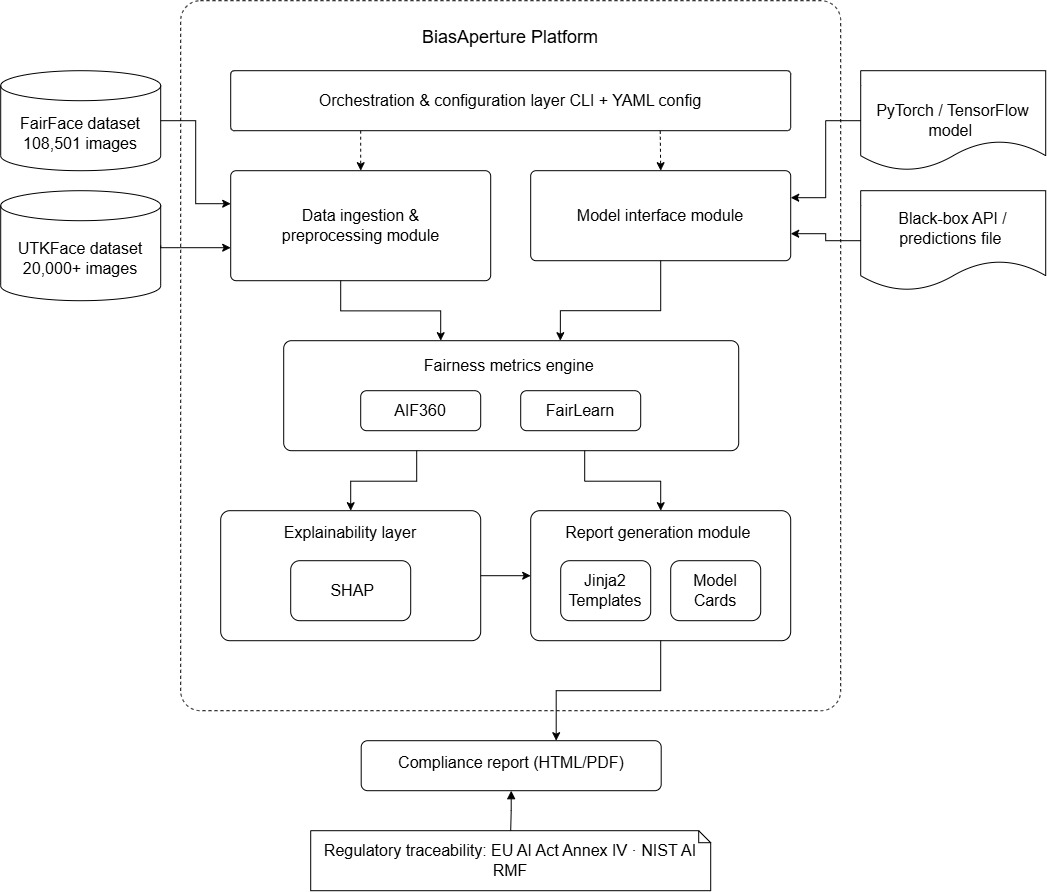
\includegraphics[width=\textwidth]{src/images/architecture_highlevel.jpg}
    \caption{BiasAperture system architecture.}
    \label{fig:architecture}
\end{figure}

\cref{tab:modules} formalises the architecture shown in \cref{fig:architecture}, listing each module alongside its primary responsibility, the functional requirements it satisfies, and the key libraries it depends on. The remainder of this section discusses each module in turn, following the order in which data and control flow through the pipeline.

\begin{table}[htbp]
    \centering
    \renewcommand{\arraystretch}{1.3}
    \caption{Architectural modules and their responsibilities.}
    \label{tab:modules}
    \begin{tabular}{p{3.2cm}p{5cm}p{4.3cm}}
        \toprule
        \textbf{Module} & \textbf{Primary Responsibility} & \textbf{Key Libraries} \\
        \midrule
        Data Ingestion and Preprocessing & Load, validate, and standardise a benchmark or custom dataset (FR-001) & OpenCV, pandas, NumPy \\
        Model Interface & Obtain predictions via direct inference or a predictions file (FR-002) & PyTorch, TensorFlow \\
        Fairness Metrics Engine & Compute subgroup and intersectional metrics with significance testing (FR-003, FR-004) & AIF360, Fairlearn, scikit-learn, SciPy \\
        Explainability Layer & Attribute a detected disparity to input features (FR-005) & \gls{shap} \\
        Report Generation & Assemble findings into a Model-Cards- and Datasheets-structured report (FR-006, FR-007) & Jinja2 \\
        Orchestration and Configuration & Coordinate the pipeline end to end behind a single entry point (FR-008, FR-009) & Python \gls{cli} \\
        \bottomrule
    \end{tabular}
\end{table}
\clearpage

\subsection{Data Ingestion and Preprocessing Module}
This module loads a selected benchmark dataset, initially FairFace and UTKFace, or a compatible custom dataset, validates image integrity, standardises image resolution and colour space via OpenCV, and aligns demographic annotation fields (race or ethnicity, perceived gender, age group) into the locked internal schema (\cref{sec:schedule}). It rejects corrupted or unreadable files and enforces that every image carries a complete, correctly typed set of demographic labels before any downstream computation proceeds.

\subsection{Model Interface Module}
This module is a thin, framework-agnostic adapter that obtains predictions from a target model without requiring internal weight access. Two integration modes are supported: direct in-process inference against a supplied PyTorch or TensorFlow model exposing a standard predict interface, and batch ingestion of a precomputed predictions file in \gls{csv} or \gls{json} format for models that cannot be executed locally. The module performs no training, fine-tuning, or weight modification of any kind.

\subsection{Fairness Metrics Computation Engine}
The analytical core of the platform. It computes per-subgroup and intersectional performance metrics (accuracy, precision, recall, \gls{f1}, false-positive and false-negative rates) and the four Core~Four disparity metrics, \gls{dpd}, \gls{eod}, \gls{eop}, and \gls{dir}, using AIF360 and Fairlearn as independent, cross-validating computational back ends: because both toolkits already implement, test, and document these metrics, the platform does not need to re-derive fairness statistics from first principles, and any discrepancy between the two backends' output on the same input surfaces an integration defect rather than a genuine result. The engine additionally performs the chi-squared significance testing and bootstrap resampling required by FR-004.

\subsection{Explainability Layer}
Motivated by the proxy-variable finding discussed in \cref{chap:litreview}, this layer applies \gls{shap} to input features associated with a disparity the metrics engine has flagged, producing feature-attribution output that helps distinguish a genuinely demographic effect from an artefact of an unrelated correlated variable such as lighting or background. Consistent with NFR-008, attribution is computed only on flagged disparities rather than across the full dataset by default.

\subsection{Report Generation Module}
This module assembles the computed metrics, statistical tests, and dataset and model provenance into a standardised, exportable \gls{html} report, structurally informed by the Model Cards and Datasheets for Datasets conventions discussed in \cref{chap:litreview}. Every metric row shows subgroup sample size, point estimate, 95\% confidence interval, and either a $p$-value or an insufficient-sample flag (FR-006), and every row is additionally traceable to its Article~10 or Annex~IV clause and its \gls{nist} \gls{ai} \gls{rmf} function (FR-007, \cref{sec:regmapping}). Because the reporting layer consumes only the already-computed metrics dictionary, it is architecturally decoupled from the computation engine, which simplifies testing and prevents a reporting defect from affecting the correctness of the underlying analysis.

\subsection{Orchestration and Configuration Layer}
A lightweight layer coordinates the pipeline end to end, dataset selection, model connection, metric selection, and report generation, behind a single entry point, and exposes a configuration file and command-line interface through which an auditor specifies the audit parameters (FR-008). The dataset's licensing terms must be displayed and explicitly acknowledged before an audit is executed (FR-009).

\section{End-to-End Workflow of the System}
\label{sec:workflow}

\cref{fig:workflow} presents the end-to-end workflow followed by the system during a single audit run, tracing the sequence of steps and decision points from initial configuration through to the generation of the final compliance report.

\begin{figure}[htbp]
    \centering
    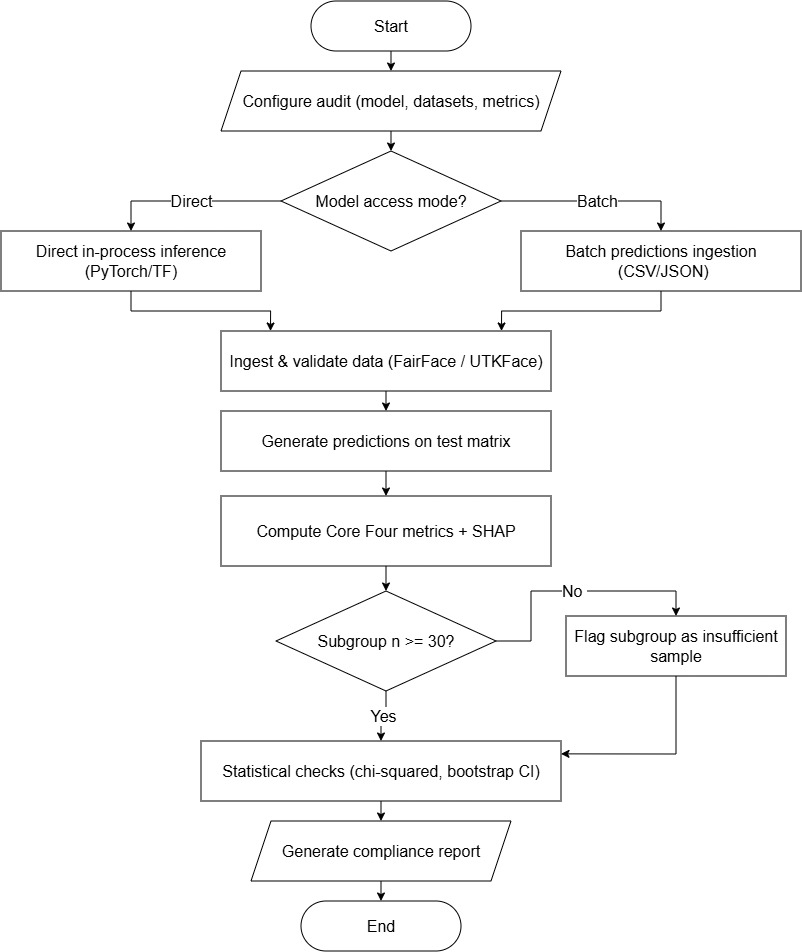
\includegraphics[width=\textwidth]{src/images/workflow_flowchart.jpg}
    \caption{BiasAperture end-to-end audit workflow.}
    \label{fig:workflow}
\end{figure}

The workflow begins with the auditor configuring the audit: specifying the benchmark or custom dataset, the target model, or a predictions file, and the metrics to compute. The system then branches on the model access mode. If a model object is supplied, predictions are obtained by direct in-process inference against the PyTorch or TensorFlow model; otherwise, predictions are obtained by batch ingestion of a precomputed CSV or JSON file. Both branches converge on a common path, in which the selected dataset, FairFace or UTKFace, is ingested and validated, and predictions are generated over the resulting test matrix.

With predictions and ground-truth labels in hand, the system computes the Core Four disparity metrics together with SHAP-based feature attribution. Before any metric is reported, each demographic subgroup is checked against the minimum sample-size guardrail: subgroups with fewer than thirty observations are flagged as an insufficient sample and excluded from the statistical checks that follow, while all other subgroups proceed directly. The remaining subgroups are then subjected to chi-squared significance testing and bootstrap confidence-interval estimation, after which the system assembles and generates the final compliance report, concluding the workflow.

\section{Design Patterns}
\label{sec:patterns}

Each pattern in \cref{tab:patterns} is tied to a specific project mechanic, either a descoping decision (\cref{sec:cutlist}) or the shared-schema contract (\cref{sec:schedule}), rather than applied for its own sake.

\begin{table}[htbp]
    \centering
    \renewcommand{\arraystretch}{1.3}
    \caption{Design patterns mapped to architectural modules.}
    \label{tab:patterns}
    \begin{tabular}{p{2cm}p{2.6cm}p{4.1cm}p{5.5cm}}
        \toprule
        \textbf{Pattern} & \textbf{Module} & \textbf{Structure} & \textbf{Rationale} \\
        \midrule
        Adapter & Model Interface & {\ttfamily\footnotesize Model\-Interface} $\to$ {\ttfamily\scriptsize Direct\-Inference\-Adapter} / {\ttfamily\scriptsize Predictions\-File\-Adapter} & Cutting direct inference (\cref{sec:cutlist}, item 4) means simply not instantiating one adapter; downstream code is unchanged \\
        Strategy & Fairness Metrics Engine & {\ttfamily\footnotesize Fairness\-Backend} $\to$ {\ttfamily\footnotesize AIF360Backend} / {\ttfamily\footnotesize Fairlearn\-Backend} & Cutting AIF360 (\cref{sec:cutlist}, item 5) is a backend swap, not a rewrite; the four metrics are interchangeable strategies \\
        Builder & Data Ingestion & {\ttfamily\footnotesize Test\-Matrix\-Builder} & Matches the multi-step curation (acquisition, integrity check, schema alignment) the module performs \\
        Factory & Report Generation & {\ttfamily\footnotesize Report\-Factory} $\to$ {\ttfamily\footnotesize HTMLReport\-Builder} & Keeps the \gls{html} report path untouched regardless of which export formats are in scope \\
        Template Method & Report Generation & {\ttfamily\footnotesize Audit\-Report} base class & Fixes the Model Cards / Datasheets section skeleton while allowing subclasses to fill format-specific hooks \\
        Facade & Orchestration & {\ttfamily\footnotesize Audit\-Orchestrator} & Hides the ingestion $\to$ interface $\to$ engine $\to$ report sequence behind one call \\
        \bottomrule
    \end{tabular}
\end{table}

\section{Regulatory Traceability Mapping}
\label{sec:regmapping}

FR-007 requires that every computed metric be mapped to a specific regulatory basis. \Cref{tab:art10} shows how the \gls{eu} \gls{ai} Act's Article~10 data-governance components map to the platform's own outputs, following the operational-verification approach of Buscemi et al.\ discussed in \cref{chap:litreview} \cite{buscemi2025assessing,euaiact2024}.

\begin{table}[htbp]
    \centering
    \renewcommand{\arraystretch}{1.3}
    \caption{Article~10 components mapped to BiasAperture outputs.}
    \label{tab:art10}
    \begin{tabular}{p{2.6cm}p{4.7cm}p{5.2cm}}
        \toprule
        \textbf{Article~10 Component} & \textbf{Technical Requirement} & \textbf{BiasAperture Evidence} \\
        \midrule
        10(2) Governance & Documentation of design choices and data origin & Dataset provenance and licensing-acknowledgement log (FR-009) \\
        10(3) Quality & Representativeness and error minimisation & Subgroup sample-size reporting and the \gls{symb:n}~$\geq 30$ insufficiency guard (NFR-003) \\
        10(4) Context & Geographical and behavioural setting adjustment & Per-dataset provenance section of the exported report \\
        10(5) Mitigation & Bias detection and disparity evidence & The four Core~Four disparity metrics with significance testing (FR-003, FR-004) \\
        \bottomrule
    \end{tabular}
\end{table}

The \gls{nist} \gls{ai} \gls{rmf}'s four functions map onto the project less as a report artefact than as a description of what the platform, and the process that built it, together accomplish. \emph{Govern} is satisfied by the scope-boundary statement (\cref{sec:cutlist}) and TA-reviewed feasibility study that establish accountability for what the platform will and will not claim to do. \emph{Map} is satisfied by the explicit demographic schema (\cref{sec:schedule}) that identifies which subgroups the platform is designed to evaluate. \emph{Measure} is the function the platform most directly operationalises: the fairness engine applies the Core~Four metrics with significance testing to determine whether a subgroup disparity meets the defined statistical thresholds. \emph{Manage} is out of the platform's diagnostic scope by design, since BiasAperture reports disparities rather than prioritising or remediating them, and this exclusion is itself stated explicitly in every generated report.

\section{Work Breakdown Structure}
\label{sec:wbs}

\Cref{tab:wbs} decomposes the project into deliverable-oriented work packages following the 100\% rule, every module in \cref{sec:modules} is covered and nothing is added outside stated scope, with leaf packages sized for a two-person team and each leaf tied either to an acceptance criterion in \cref{chap:requirements} or to a module in \cref{sec:modules}. Ownership is tagged \emph{Together} where a package requires shared judgement or iteration, or \emph{Stream~A} / \emph{Stream~B} where it can proceed solo; named assignment of which team member takes which solo stream remains open at time of writing and will be settled by demonstrated preference rather than fixed in advance.

\begin{table}[htbp]
    \centering
    \renewcommand{\arraystretch}{1.3}
    \caption{Work breakdown structure.}
    \label{tab:wbs}
    \begin{tabular}{p{0.9cm}p{6.4cm}p{2.2cm}}
        \toprule
        \textbf{ID} & \textbf{Work Package} & \textbf{Ownership} \\
        \midrule
        1.1 & Project management: feasibility review, acceptance-criteria lock, schema lock, submission and defence prep & Together \\
        1.2 & Classifier selection and model interface: baseline confirmation, \texttt{ModelInterface} abstraction, predictions-file ingestion path & Together \\
        1.3 & Stream~A, test-matrix construction: dataset acquisition and integrity check, inference run, schema curation, stratified development subset & Stream~A \\
        1.4 & Stream~B, report scaffolding: \gls{html} and Jinja2 template, Model Cards / Datasheets structure, hand-written mock metrics dictionary & Stream~B \\
        1.5 & Statistical detection engine: backend integration, four disparity metrics, chi-squared testing, bootstrap confidence interval, sample-size guard & Together \\
        1.6 & Integration: Stream~A output into the detection engine, mock-to-real swap of Stream~B's report against real findings, orchestration module & Together \\
        1.7 & Verification and validation: runtime targets, report-completeness rule, case-study run & Together \\
        1.8 & Documentation and delivery: scope-boundary statement, final report, submission package & Together \\
        \bottomrule
    \end{tabular}
\end{table}

\section{Project Plan and Schedule}
\label{sec:schedule}

The work packages in \cref{tab:wbs} are restructured for concurrency rather than executed as a strict sequence, so that neither team member is idle while the other's phase is blocking. \Cref{fig:gantt} shows the resulting eight-week schedule.

\begin{figure}[htbp]
    \centering
    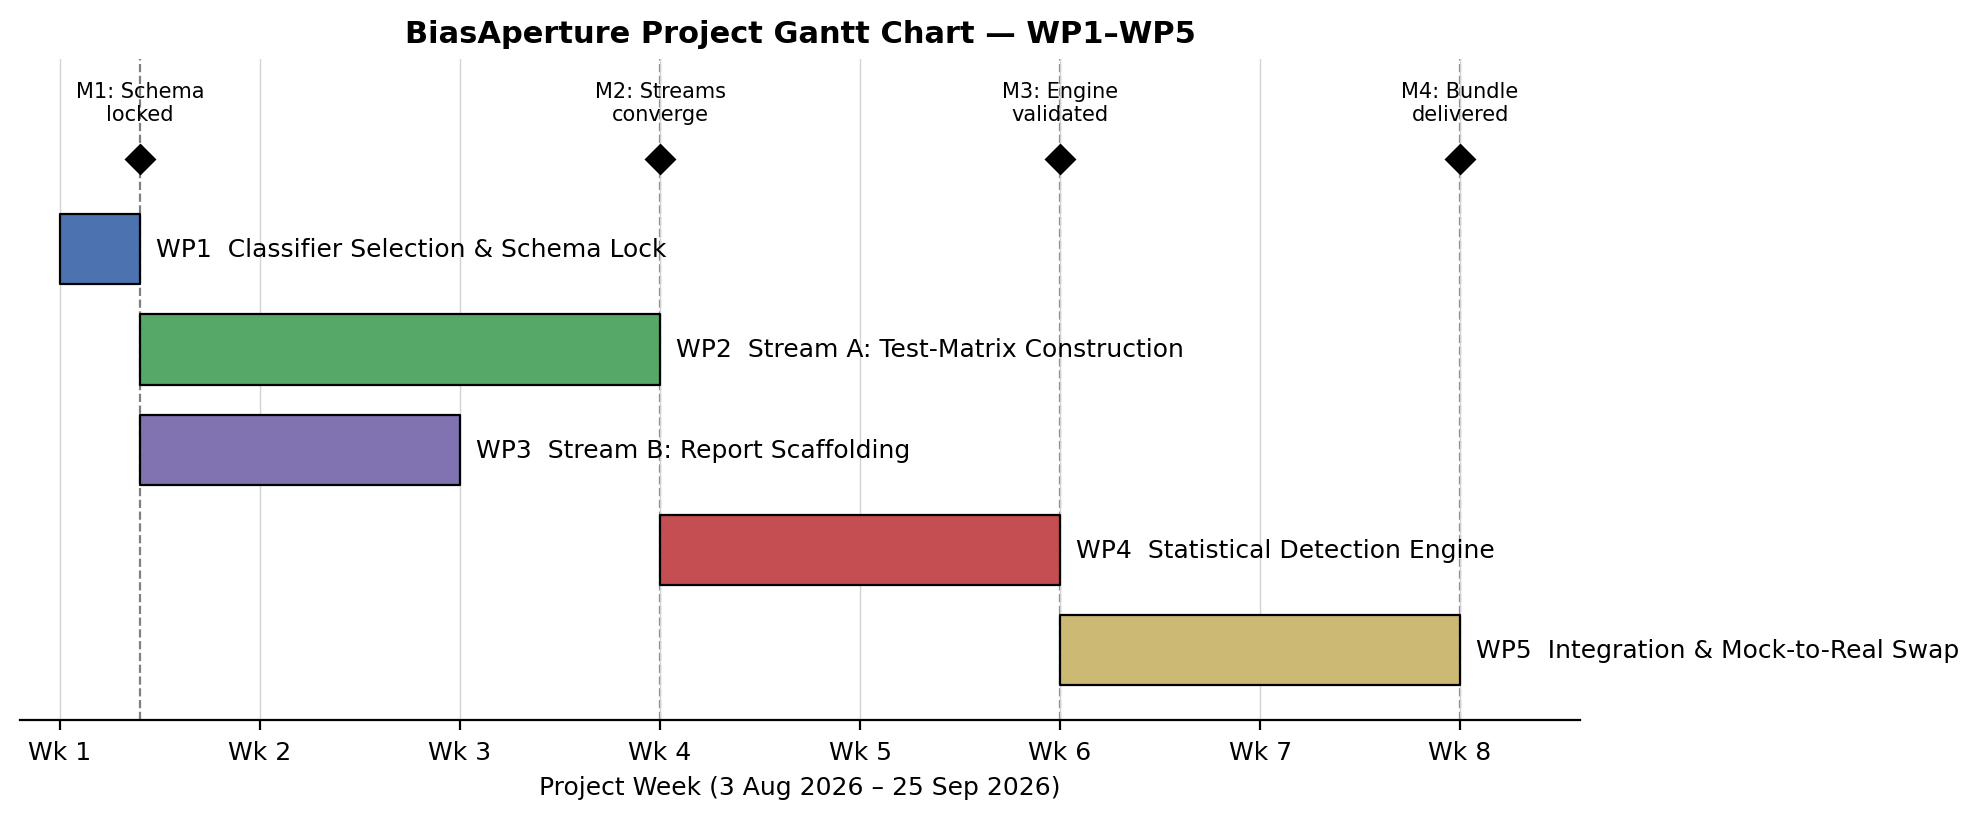
\includegraphics[width=\textwidth]{src/images/gantt.png}
    \caption{BiasAperture project schedule, work packages WP1--WP5.}
    \label{fig:gantt}
\end{figure}

WP1, \emph{Classifier Selection and Schema Lock}, is a short, foundational, jointly worked phase that fixes the classifier baseline and the internal demographic schema every later module must honour: an \texttt{image\_id}, race, gender, and age subgroup fields, predicted and true labels, and, for the detection engine's output, metric name, point estimate, confidence bounds, $p$-value, and subgroup sample size. Its completion is Milestone~M1, \emph{schema locked}.

With the schema fixed, WP2 (Stream~A, test-matrix construction) and WP3 (Stream~B, report scaffolding) begin immediately and run in parallel rather than sequentially: Stream~A curates the FairFace-based dataset and predictions file against the locked schema while Stream~B builds the \gls{html} report template and Model Cards / Datasheets structure against a hand-written mock metrics dictionary that validates against the same field set. Both streams converge at Milestone~M2.

WP4, the \emph{Statistical Detection Engine}, is the joint convergence phase: it consumes Stream~A's schema-aligned test matrix as input and produces the schema-shaped metrics dictionary Stream~B's report template already expects, running faster than it otherwise would because both interfaces were fixed before this phase began. Its completion, Milestone~M3, is the point at which the engine is validated end to end.

WP5, \emph{Integration and Mock-to-Real Swap}, replaces Stream~B's mock metrics dictionary with the detection engine's real output, a short, mechanical step precisely because the template was built against an identical schema in week one, and completes with the final case-study audit and report bundle at Milestone~M4.

\section{Descoping Strategy}
\label{sec:cutlist}

The scope defined in \cref{chap:requirements} is deliberately fuller than a two-person, eight-week timeline is guaranteed to accommodate without slippage. Rather than discover a descoping order under deadline pressure, \cref{tab:cutlist} fixes it in advance.

\begin{table}[htbp]
    \centering
    \renewcommand{\arraystretch}{1.3}
    \caption{Descoping order if the project falls behind schedule.}
    \label{tab:cutlist}
    \begin{tabular}{p{0.6cm}p{3.6cm}p{7.3cm}}
        \toprule
        \textbf{\#} & \textbf{Cut} & \textbf{Rationale} \\
        \midrule
        1 & Web \gls{ui}, keep \gls{cli} only & Pure user-experience layer; no bearing on the fairness-engineering core \\
        2 & UTKFace, keep FairFace only & The architecture already anticipates this; UTKFace's DEX-estimated label noise is an already-documented risk \\
        3 & \gls{pdf} export, keep \gls{html} only & \gls{html} alone satisfies the standardised, exportable report requirement and the Model Cards / Datasheets structure \\
        4 & Direct in-process inference, keep predictions-file ingestion only & The simpler mode; removes \gls{gpu} and dependency-version risk entirely, and a public pretrained checkpoint and inference script make it sufficient for the case study \\
        5 & AIF360, keep Fairlearn only & Last resort; Fairlearn alone computes all four Core~Four metrics, but this is the only cut that measurably weakens the cross-validated, methodologically defensible claim \\
        \bottomrule
    \end{tabular}
\end{table}

The non-negotiable core that is never cut, regardless of timeline pressure, is: data ingestion, one model interface, the fairness engine, one report format, and the scope-boundary statement itself.

\section{Verification and Validation Strategy}

Statistical correctness is verified before any real-data run: the chi-squared and bootstrap-resampling routines are unit-tested against known reference values first, so that a defect in the significance-testing code is caught independently of whatever pattern happens to appear in a real audit's results. Both streams' outputs are additionally schema-validated against the locked field set from \cref{sec:schedule}, directly defusing the risk that independent development on either side silently drifts and breaks the WP5 integration step. Version control follows a feature-branch-per-stream model off a \texttt{main} branch holding only the locked schema and module skeletons, with review at the WP4 convergence point before merge. Runtime and report-completeness are validated against the acceptance criteria already fixed in \cref{chap:requirements} (NFR-002, NFR-003, NFR-004), and the case study itself, a FairFace-trained ResNet-34 baseline evaluated on all four Core~Four metrics, exercises the full pipeline end to end as the platform's own validation instance.
